\chapter{Introduction}

\section{Quantum Chromodynamics}

Early theoretical work in nuclear physics, after the discovery of the neutron, focused on establishing the theory of the strong force responsible for binding together protons and neutrons. The earliest model, that of Yukawa, relied on the exchange of a massive boson (the $\pi$ meson). Later experiments looking at harder interactions between nucleons showed that these processes could produce a large variety of hadrons, pointing to a much richer structure within protons and neutrons. Thus it became necessary to think beyond the model of the nuclear force (protons and neutrons exchanging pions), and instead look at the more fundamental strong force which gives rise to the structure and interaction of all hadrons. In the 1960s the quark model was developed and successfully explained the multiple observations of new hadrons being created in collider experiments by supposing that hadrons were not fundamental particles, but rather composed of quarks.

Quantum Chromodynamics (QCD) is the fundamental theory of the strong force and describes the interactions between quarks which is mediated by gluons. Quarks come in 6 flavors: up, down, strange, charm, bottom, and top. All quarks have a fractional electric charge (either $\pm \frac{1}{3}e$ or $\pm \frac{2}{3}e$). Quarks carry a color (red, green, or blue) and are bound by gluons into groups of three (baryons) or two (mesons). Baryons and mesons have no color, in baryons the three colors add up in a way that is color neutral while in mesons the one quark carries a color and the antiquark carries an anticolor. 

Deep inelastic scattering experiments at SLAC further probed the structure of nucleons and showed that they were composed of three spin-$1/2$ particles. These measurements confirmed the quark model and showed that quarks were real particles within hadrons. DIS experiments also suggested other peculiar and (at the time) unexpected behaviors in quarks. When bound quarks are probed at higher energy scales they behave as if they were free. In fact it is the case with quarks that with large momentum exchange the coupling between quarks and gluons is weak and we can treat QCD perturbatively. However as the energy scale decreases the coupling becomes stronger and perturbation theory no longer applies. This property of QCD is called asymptotic freedom and was discovered in 1973 by Gross, Wilczek, and Politzer for which they were awarded the Nobel Prize in 2004. Asymptotic freedom arises in QCD because it is a non-Abelian gauge theory. There is screening of the color charge of quarks by the vacuum, however there is also anti-screening from charged spin-1 gluons. The value of the coupling in QCD can be represented by the $\beta$ function, for QCD it can be shown that to lowest order $\beta(g)$ is propotional to $-(\frac{11}{2} - \frac{n}{3})$ where n is the number of quarks. For QCD, with 8 gluons and 3 colors, the anti-screening from the gluons overcomes the screening of the quarks and thus the theory is asyptotically free. Figure~\ref{fig:a_free} shows experimental estimates of $\alpha_S$ as well as the scale of the momentum exchange. Experimental results are in agreement with the predictions of asymptotic freedom. 

\begin{figure}[htbp]
\begin{center}
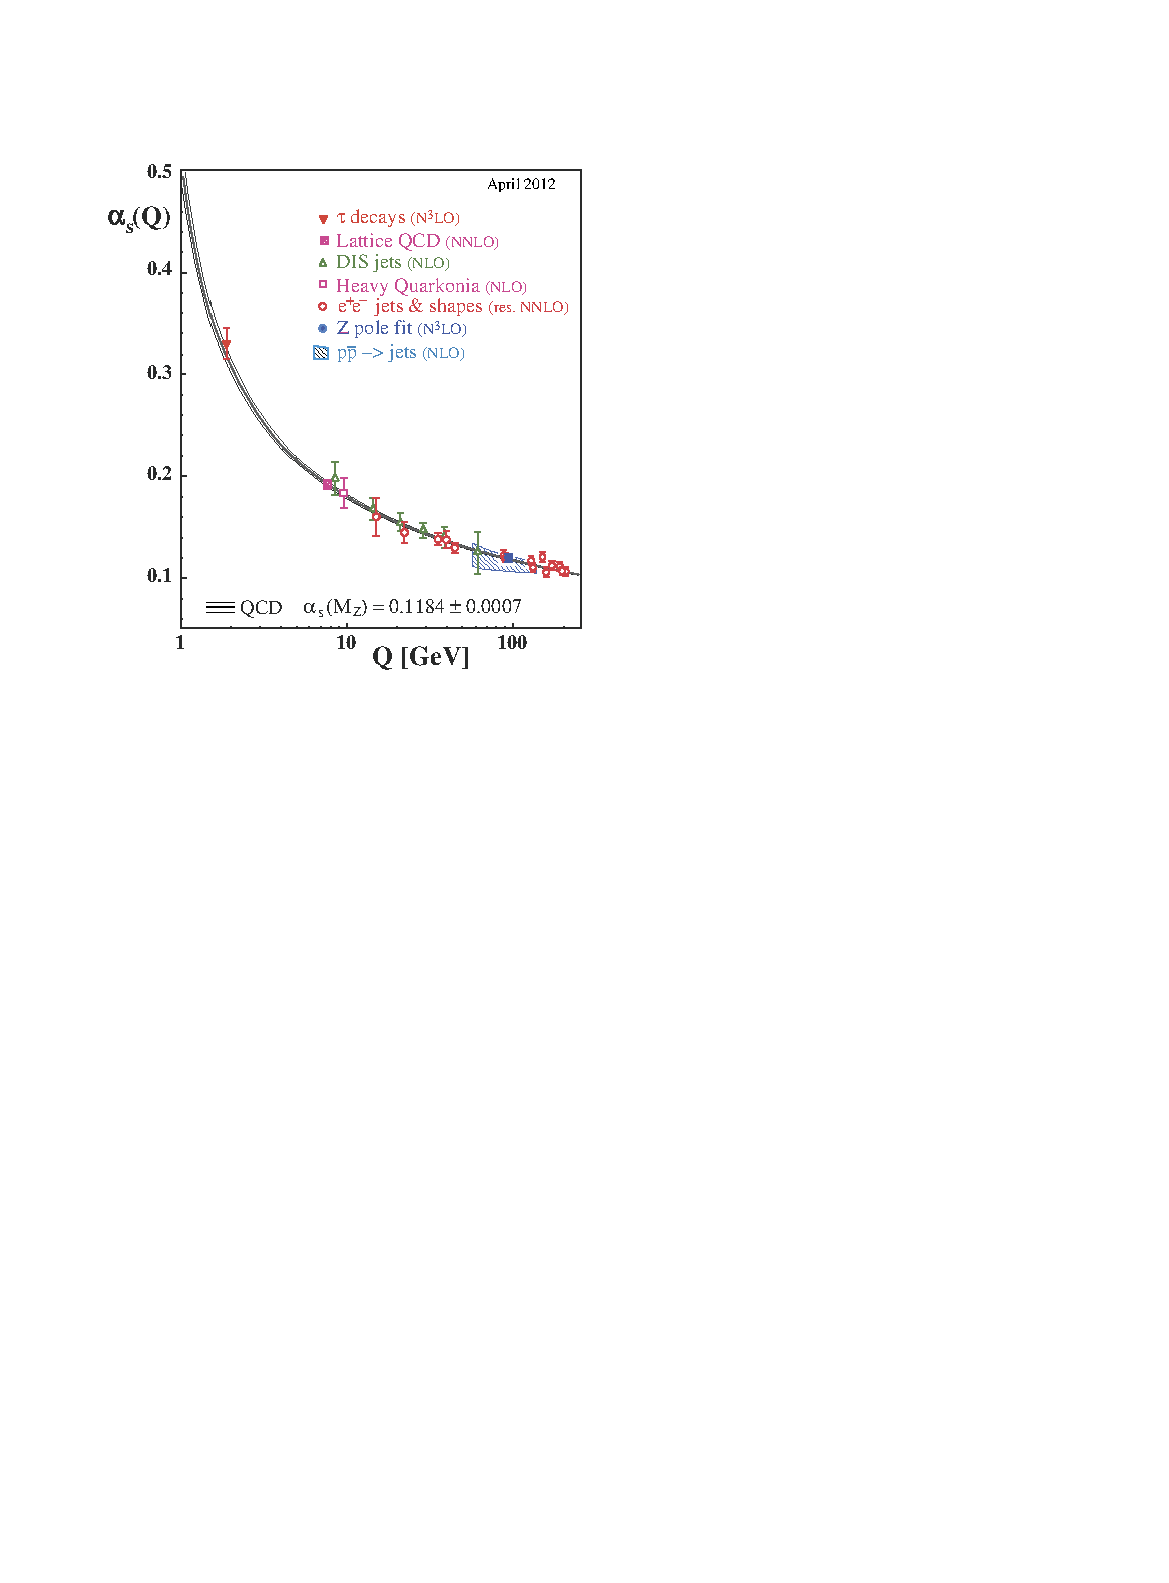
\includegraphics[scale=1.3]{Plots/Intro/asymp_free.pdf}
\end{center}
\caption[Asymptotic Freedom]{Several measurements of the strong coupling constant $\alpha_S$ showing how it varies with energy scale. Decreasing coupling strength as the interaction energy goes up is consistent with predictions of asymptotic freedom}
\label{fig:a_free}
\end{figure}

Within baryons and mesons quarks are bound in colorless states, and as explained above, at short distance scales the coupling between the quarks and gluons in weak and we can treat the interaction of quarks perturbatively. However, when we attempt to remove a quark from a hadron lattice QCD calculations show the potential increases linearly with distance. Eventually the energy put into this hypothetical system increases to a high enough point that a new quark anti-quark pair is created from the vacuum and we end up with two hadrons. This property of QCD, that quarks and gluons remain bound in colorless states, we refer to as confinement. 

Confinement and asymptotic freedom are two of the most interesting properties associated with QCD, and are responsible for many of the interesting phenomena within the strong interaction. As we dive deeper into QCD we will next explore the QCD phase diagram, and look for evidence of confinement being broken.  

\section{QCD Phase Diagram and Deconfinement}

At low temperatures lattice calculations show that quarks are confined within hadrons, we will now turn our attention to the properties of quark matter under more extreme conditions. Lattice calculations also predict a rich phase structure in QCD beyond just what we observe in low temperature hadronic matter. As we increase the temperature and density of nuclear matter it is predicted that quarks and gluons are deconfined from their hadronic states. We call this hot dense state of matter with strongly interacting free quarks and gluons the Quark Gluon Plasma (QGP). Conditions in the universe allowed for QGP to exist up until about $10^{-5}$s after the Big Bang. There is also the chance that colder deconfined matter could exist within neutron stars.

Figure~\ref{fig:qcd_phase} shows an illustration of the QCD phase diagram. Nuclear matter exists in the lower right part of the figure, inside nuclei the temperatures are low and the average net baryon number is high. The figure also shows the regions of the phase diagram which are accesible to various experiements which we will discuss further in upcoming sections. Also of note is that the phase transition from QGP to hadronic matter can be either a first order or second order phase transition and that there is postulated to be a critical point in the QCD phase diagram. The search for the QCD critical point is an area of active research, but is beyond the scope of this dissertation. 

\begin{figure}[htbp]
\begin{center}
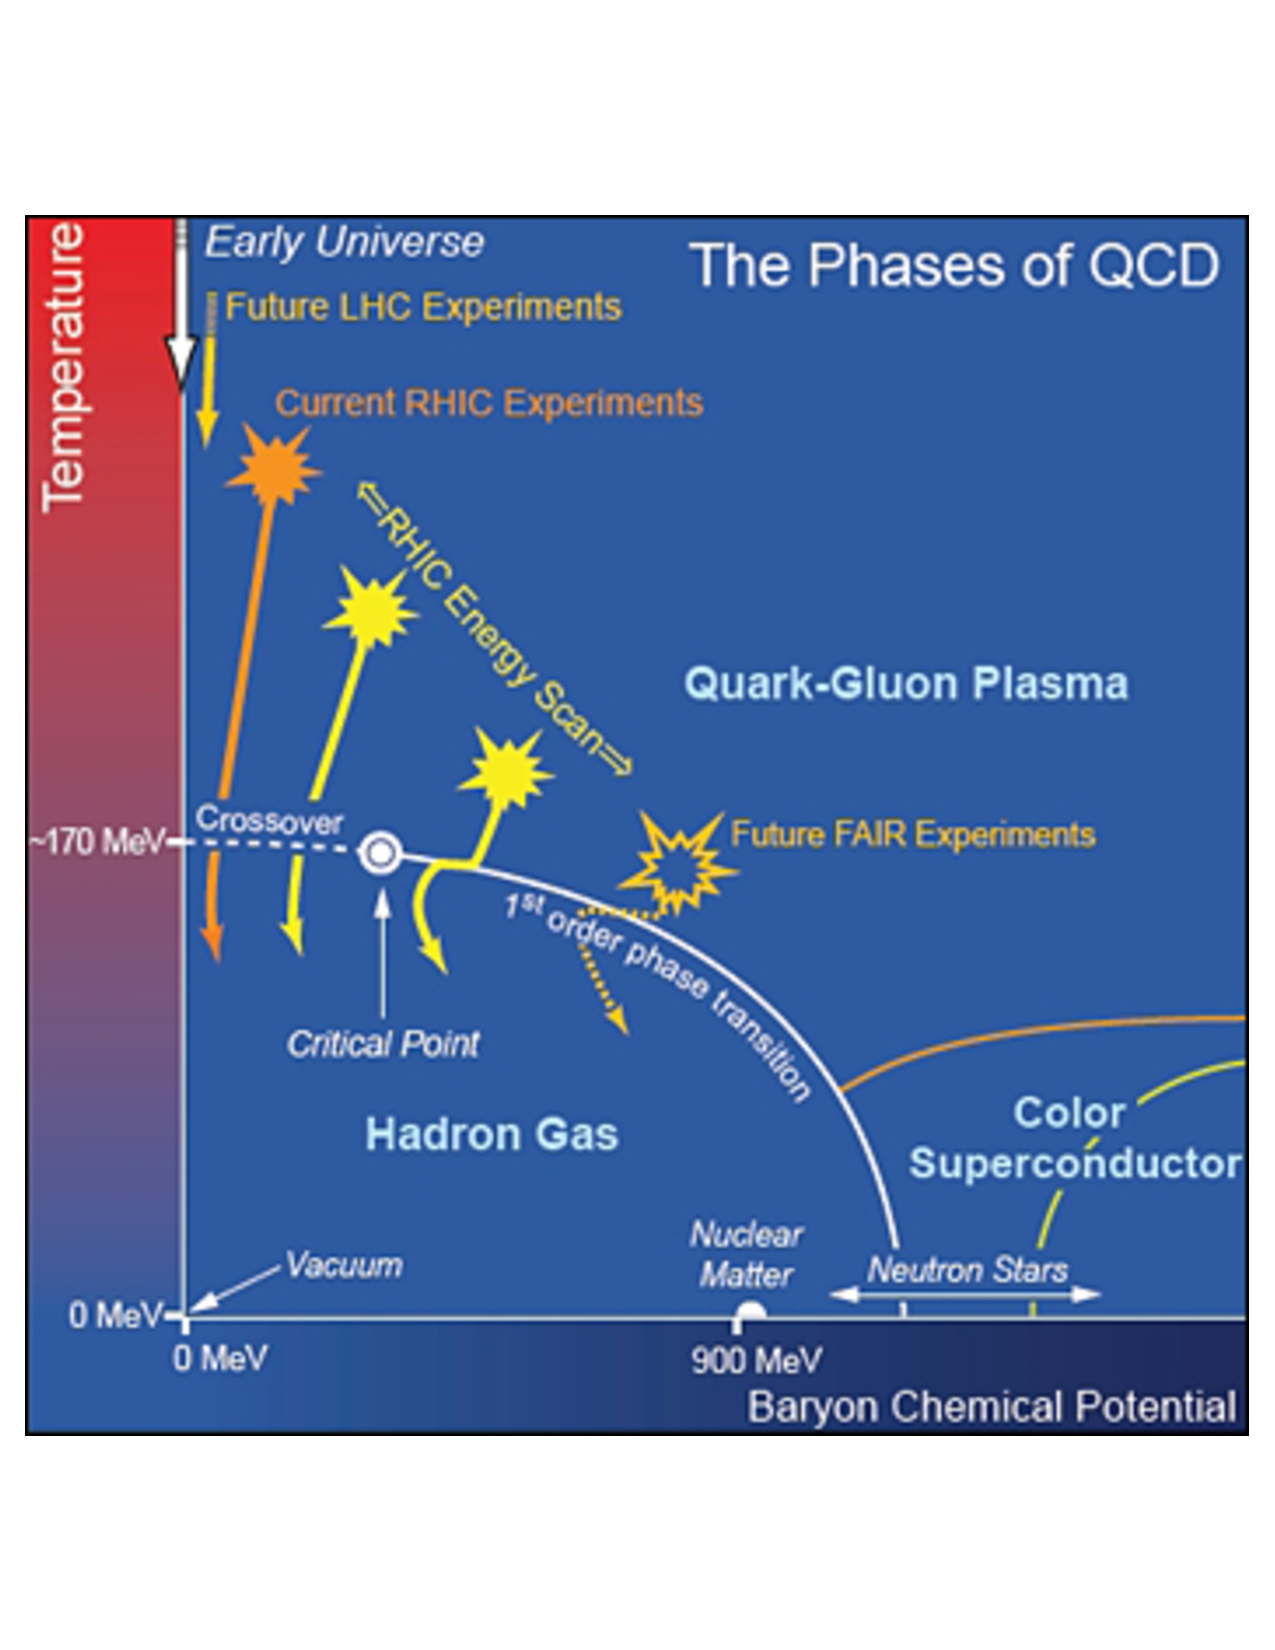
\includegraphics[scale=0.5]{Plots/Intro/qcd_phase.pdf}
\end{center}
\caption[QCD Phase Diagram]{Illustration of the QCD phase diagram showing the various regimes as well as the reach of current experiments.}
\label{fig:qcd_phase}
\end{figure}

The critical behavior in QCD can be seen in the bulk thermodynamic properties of QGP around the critical temperature $T_c$. Figure~\ref{fig:pressure} shows the quantity $p/T^4$ as a function of temperature for various quark flavor combinations. At the critical temperature there is a transition from hadronic to partonic degrees of freedom which is seen in the large jump in $p$. At high temperatures the medium behaves as an ideal gas. The increase in degrees of freedom is taken as evidence that the phase transition in QCD coicides with the onset of deconfinement.

\begin{figure}[htbp]
\begin{center}
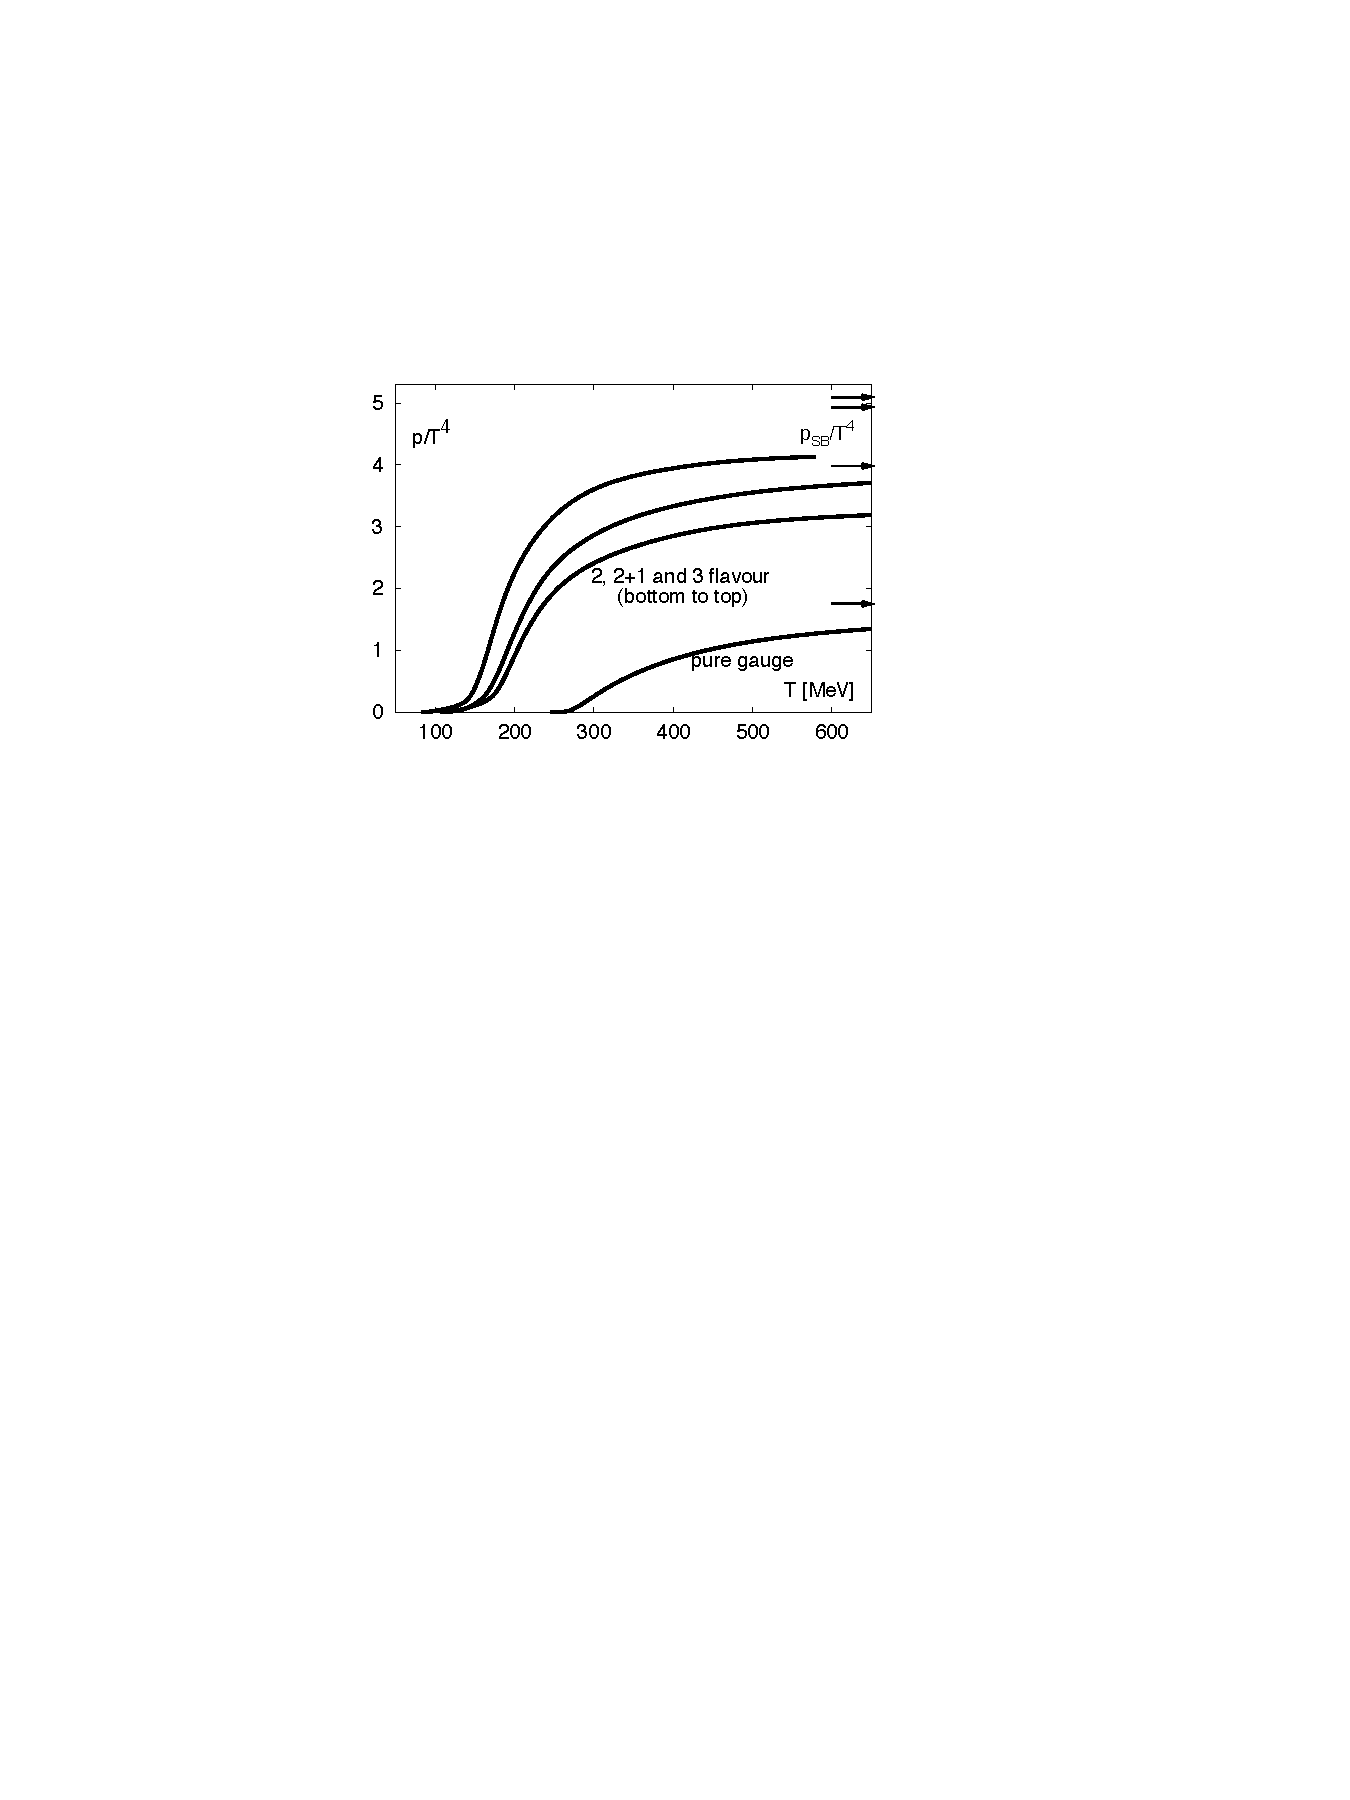
\includegraphics[scale=1.0]{Plots/Intro/pressure.pdf}
\end{center}
\caption[$p/T^4$ Calculations]{Calculations of $p/T^4$ in QCD for various numbers of quark flavors. Large jump near $T_c$ is the result of an increase in the number of degrees of freedom in the medium and is caused by the deconfinement of hadronic matter.}
\label{fig:pressure}
\end{figure}

\section{Experiments on QGP}

\section{Heavy Flavor Probes}

\section{Two Particle Correlations}
